\documentclass{article}
\usepackage[paperwidth=7.16in,paperheight=4.55in,margin=0.06in]{geometry}
\usepackage{amsmath}
\usepackage{amssymb}
\usepackage{tikz}
\usetikzlibrary{arrows.meta,positioning,calc}
\pagestyle{empty}
\setlength{\parindent}{0pt}

% Restrained manuscript palette: gray for real features, blue for complex
% features, and soft beige/violet for the interaction modules.
\definecolor{realfill}{RGB}{246,246,246}
\definecolor{realedge}{RGB}{91,91,88}
\definecolor{complexfill}{RGB}{237,246,250}
\definecolor{complexedge}{RGB}{54,102,135}
\definecolor{interactionfill}{RGB}{249,246,238}
\definecolor{interactionedge}{RGB}{142,112,61}
\definecolor{residualfill}{RGB}{247,244,250}
\definecolor{residualedge}{RGB}{104,82,128}
\definecolor{textgray}{RGB}{55,55,53}

\begin{document}
\centering
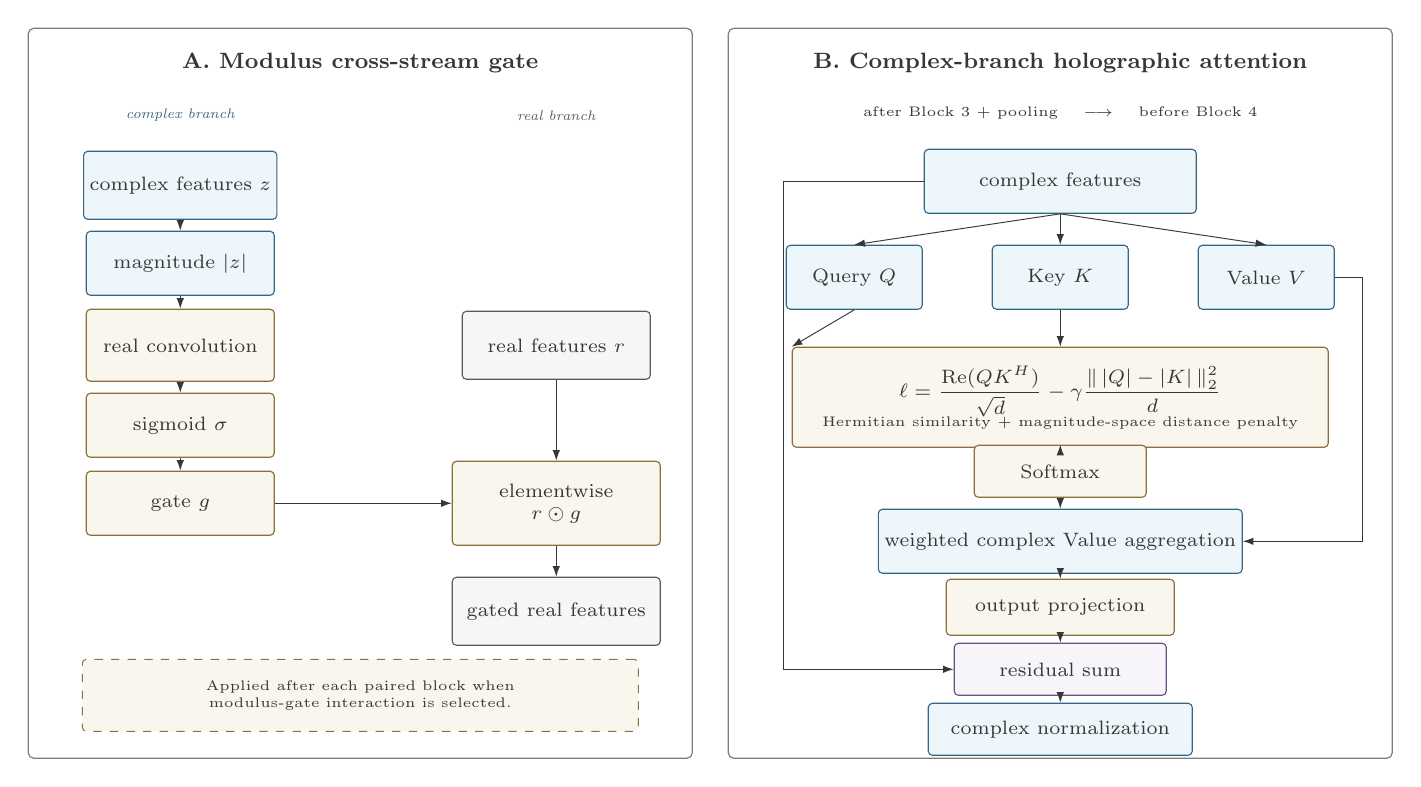
\begin{tikzpicture}[
  x=1in,y=1in,
  font=\scriptsize,
  text=textgray,
  >=Latex,
  arrow/.style={-{Latex[length=1.35mm,width=0.95mm]},line width=0.34pt,draw=textgray},
  panel/.style={rounded corners=2pt,draw=textgray!65,fill=white,line width=0.44pt},
  realbox/.style={rounded corners=1.5pt,draw=realedge,fill=realfill,line width=0.40pt,
    align=center,inner sep=2.2pt},
  complexbox/.style={rounded corners=1.5pt,draw=complexedge,fill=complexfill,line width=0.40pt,
    align=center,inner sep=2.2pt},
  interactionbox/.style={rounded corners=1.5pt,draw=interactionedge,fill=interactionfill,line width=0.42pt,
    align=center,inner sep=2.2pt},
  residualbox/.style={rounded corners=1.5pt,draw=residualedge,fill=residualfill,line width=0.42pt,
    align=center,inner sep=2.2pt},
  annotation/.style={rounded corners=1.5pt,draw=interactionedge,fill=interactionfill,dashed,line width=0.36pt,
    align=center,inner sep=2.4pt,font=\tiny},
  title/.style={font=\footnotesize\bfseries,align=center},
  note/.style={font=\tiny,align=center,text=textgray},
  branchnote/.style={font=\tiny\itshape,align=center}
]

% The panels share the same footprint and internal margins.
\node[panel,minimum width=3.32in,minimum height=3.65in] (panelA) at (-1.75,0.08) {};
\node[panel,minimum width=3.32in,minimum height=3.65in] (panelB) at (1.75,0.08) {};

% -------------------------------------------------------------------------
% A. Modulus cross-stream gate.
% -------------------------------------------------------------------------
\node[title] at (-1.75,1.73) {A. Modulus cross-stream gate};
\node[branchnote,text=complexedge] at (-2.65,1.47) {complex branch};
\node[branchnote,text=realedge] at (-0.77,1.47) {real branch};

% Complex-to-gate lane. The gate is aligned with the real-stream
% multiplication so the one-way cross-stream handoff is explicit.
\node[complexbox,minimum width=0.94in,minimum height=0.34in] (az) at (-2.65,1.12)
  {complex features $z$};
\node[complexbox,minimum width=0.94in,minimum height=0.32in] (amag) at (-2.65,0.73)
  {magnitude $|z|$};
\node[interactionbox,minimum width=0.94in,minimum height=0.36in] (aconv) at (-2.65,0.32)
  {real convolution};
\node[interactionbox,minimum width=0.94in,minimum height=0.32in] (asig) at (-2.65,-0.08)
  {sigmoid $\sigma$};
\node[interactionbox,minimum width=0.94in,minimum height=0.32in] (agate) at (-2.65,-0.47)
  {gate $g$};
\foreach \a/\b in {az/amag,amag/aconv,aconv/asig,asig/agate}
  {\draw[arrow] (\a.south) -- (\b.north);}

% Real-stream lane. Only this lane is modulated by the complex-derived gate.
\node[realbox,minimum width=0.94in,minimum height=0.34in] (ar) at (-0.77,0.32)
  {real features $r$};
\node[interactionbox,minimum width=1.04in,minimum height=0.42in] (amul) at (-0.77,-0.47)
  {elementwise\\$r\odot g$};
\node[realbox,minimum width=1.04in,minimum height=0.34in] (aout) at (-0.77,-1.01)
  {gated real features};
\draw[arrow] (ar.south) -- (amul.north);
\draw[arrow] (agate.east) -- (amul.west);
\draw[arrow] (amul.south) -- (aout.north);
\node[annotation,minimum width=2.78in,minimum height=0.36in,text width=2.54in] at (-1.75,-1.43)
  {Applied after each paired block when modulus-gate interaction is selected.};

% -------------------------------------------------------------------------
% B. Holographic attention.
% -------------------------------------------------------------------------
\node[title] at (1.75,1.73) {B. Complex-branch holographic attention};
\node[note,text width=2.84in] at (1.75,1.48)
  {after Block 3 + pooling $\;\longrightarrow\;$ before Block 4};

\node[complexbox,minimum width=1.36in,minimum height=0.32in] (bx) at (1.75,1.14)
  {complex features};
\node[complexbox,minimum width=0.68in,minimum height=0.32in] (bq) at (0.72,0.66)
  {Query $Q$};
\node[complexbox,minimum width=0.68in,minimum height=0.32in] (bk) at (1.75,0.66)
  {Key $K$};
\node[complexbox,minimum width=0.68in,minimum height=0.32in] (bv) at (2.78,0.66)
  {Value $V$};
\draw[arrow] (bx.south) -- (bq.north);
\draw[arrow] (bx.south) -- (bk.north);
\draw[arrow] (bx.south) -- (bv.north);

\node[interactionbox,minimum width=2.68in,minimum height=0.50in] (blogits) at (1.75,0.06)
  {$\ell=\dfrac{\operatorname{Re}(QK^{H})}{\sqrt d}
    -\gamma\dfrac{\lVert\,|Q|-|K|\,\rVert_2^2}{d}$\\[-1pt]
    {\tiny Hermitian similarity $+$ magnitude-space distance penalty}};
\draw[arrow] (bq.south) -- (blogits.north west);
\draw[arrow] (bk.south) -- (blogits.north);

\node[interactionbox,minimum width=0.86in,minimum height=0.26in] (bsoft) at (1.75,-0.31)
  {Softmax};
\node[complexbox,minimum width=1.62in,minimum height=0.32in] (bagg) at (1.75,-0.66)
  {weighted complex Value aggregation};
\node[interactionbox,minimum width=1.14in,minimum height=0.28in] (bproj) at (1.75,-0.99)
  {output projection};
\node[residualbox,minimum width=1.06in,minimum height=0.26in] (badd) at (1.75,-1.30)
  {residual sum};
\node[complexbox,minimum width=1.32in,minimum height=0.26in] (bnorm) at (1.75,-1.60)
  {complex normalization};
\draw[arrow] (blogits.south) -- (bsoft.north);
\draw[arrow] (bsoft.south) -- (bagg.north);
\draw[arrow] (bv.east) -- ++(0.14,0) |- (bagg.east);
\draw[arrow] (bagg.south) -- (bproj.north);
\draw[arrow] (bproj.south) -- (badd.north);
\draw[arrow] (badd.south) -- (bnorm.north);
% Skip path from the complex input to the residual sum.
\draw[arrow] (bx.west) -- ++(-0.70,0) |- (badd.west);
\end{tikzpicture}

\vspace{0.05in}
\begin{minipage}{7.00in}
\scriptsize
\textbf{Figure 5.} Implemented interaction mechanisms. The modulus gate derives a sigmoid gate from complex-feature magnitudes and applies it multiplicatively to the corresponding real-stream features after each paired block. Holographic attention operates only on the complex branch after the third pooled stage, combining Hermitian query--key similarity with a magnitude-distance penalty before complex value aggregation.
\end{minipage}
\end{document}
